\section{Real-time implementation and preliminary results}
\label{sec:rt}

There are two components to the application:
the static GTFS~schedule and network data,
and the real-time modeling and prediction.
We chose \verb+Rcpp+ to develop our program,
giving us the advantages of an R~package for data manipulation 
(notably \verb+RSQLite+ and \verb+dplyr+)
and distribution, 
as well as the speed and memory management capabilities of \verb|C++|. 
As a result, all of the following has been implemented in the R package
\verb+transitr+, available on Github (\url{https://github.com/tmelliott/transitr}).
Here our focus is on the real-time aplication, so we are only discussing the real-time 
features of model's implementation.

The general structure of the main function is:
\begin{enumerate}
\item Load GTFS data from database
\item Indefinitely repeat when new data recieved \ldots
\begin{enumerate}
    \item Update or create new vehicle objects from new data
    \item Run particle filter on each vehicle to estimate update state
    \item Collect travel time information for each vehicle for any completed roads
    \item Update road network with any completed road segments
    \item Generate ETAs for vehicles
    \item Write ETAs to extended Google Protobuf binary file for distribution
\end{enumerate}
\end{enumerate}

The main concern is speed: 
we desire ETAs to be available as soon as possible after obtaining the data.
To do this, we use raw pointers to read-only GTFS objects,
and particles are only copied when resampling is required.
This is also why we chose to use protobuf as the output format,
since this is fast to write and distribute.
Steps 2b--e are performed in parallel, 
which in our test environment of a virtual machine with 8~cores, 
significantly speeds up computation.


As far as results, we have two categories:
implementation and faesibility,
and model performance;
we do not have any complex arrival time estimation method,
so no results for that are shown here.


The simulations we discuss here use a subset of real data from 8~October, 2018.
This allows us to run the model with different parameters over the same data.
The parameters varied were the number of particles and system noise $\sigma^2$.
The primary goal is to reduce the rate of degeneration and ``losing'' the bus 
(i.e., no particles are near the observed location),
and reducing the variance of parameter estimates; here we use vehicle speed as the example.


The one parameter we can determine from the data is GPS error, $\epsilon^2$,
by looking at the distance between observations and the shape.
Figure~\ref{fig:gps_dist} shows the distribution of distance between the vehicle
observation and the \emph{nearest point on the path}.
Due to the way the observations are reported, 
many observations will be ``exactly'' on the route at a bus stop,
and we need to ignore these.

\begin{figure}[tb]
    \centering
    % \includegraphics[width=0.7\textwidth]{figures/04_model_results_gps.pdf}
    \caption{The distance between the observation and the nearest point on the shape.}
    \label{fig:gps_dist}
\end{figure}



\subsection{Program Timings}
\label{sec:timings}

During development of our application,
our primary concert was the computational faesibility of a particle filter.
For each iteration, 
the timings of the individual components in 2a--f above are recorded.
Since the number of vehicles traveling at any given time changes throughout the day,
we used the average timings from 13:45--14:00 to compare.


Figure~\ref{fig:timings} shows the timing results for varying number of particles.
Nothing too exciting going on here, 
except that writing ETAs takes up the largest chunk of time,
as this involves calculating quantiles which require the estimated ETAs to be sorted,
which is computationally demanding. 
The vehicle update takes the second longest time,
and involves copying particles during the update resampling step.
Finally, predicting the ETAs is pretty quick.
The remaining parts of the application take negligible time,
and all run on a single core to avoid mutex locks.



\begin{figure}[tb]
    \centering
    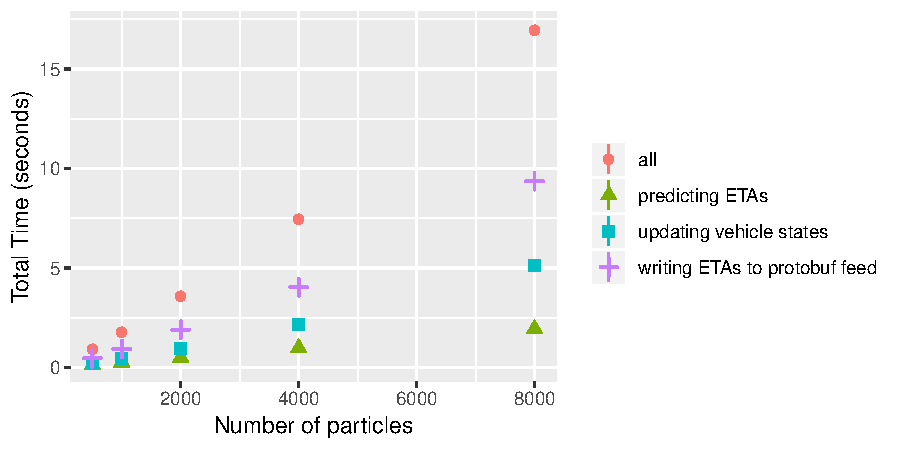
\includegraphics[width=0.7\textwidth]{figures/04_model_results_timing.pdf}
    \caption{The timings for various parts of the application, and overall. %
        The trend is approximately linear with the number of particles.}
    \label{fig:timings}
\end{figure}




\subsection{Model performance}
\label{sec:model_perf}

To check the model results, 
we need to realise that we are not trying to accurately predict
future locations of the vehicle,
but instead are trying to use a sequence of GPS positions to infer travel
times along intermediate roads.
Therefore, several tools used to assess the validity of a particle filter
are unnecessary.
Instead, we will be comparing the rate of degeneration 
(i.e., the particle sample loses the actual bus and needs to be reinitialized)
and the mean distance between the state estimate and the observation; 
we will use the distance between the observation and the route (cross track distance) 
to determine how well the posterior distribution fits the data---%
if the ratio between the CTD and RMSE is large,
then the fit is ``bad''.
[We also explore the uncertainty of travel time estimates,
as well as the variability between consecutive buses]\footnote{assuming we can get the results in time}.



From the Figure~X, 
we see a trade-off between some of the parameters.
Larger values of GPS error decrease the degeneration rate
as well as the rate of resampling (which increases speed);
however, the cost of this is that the mean distance between the posterior distribution
and the observed location increases, giving a less precise estimate of the vehicle's state.
Conversely, the system noise does not have the same effect,
and only slightly effects the values.


So the main way to determine how well everything is working is to look 
at the RMSE of ETAs over time.



% How we implement it, choice of software (Rcpp = R + C++).
% R: dealing with data structures is easier, maintainability, interfacing
% C++: speed

% Overall structure:
% - load
% - fetch positions
% - initialize or mutate+update
% - update network
% - make ETA predictions (vehicle state + network state)

% Some of the key things:
% - minimise copy, parallelisation using OMP
% - moving as much computation ``outside'' of the main loop as possible
%   (e.g., ``pre''-predict vehicle/network states so only update required)
%   so ETAs are generated ASAP after retrieving data
% - keeping the GTFS database up-to-date by fetching new data each morning
% - distribution - a cloud database vs a single protobuf file with everything 
%   (maintenance/reliability/speed/size)

